\chapter{背景介绍}
\section{图的三大范式}
属性图、RDF图和超图常常被并称为定义图结构的三大模型范式。

\subsection{属性图}
属性图是最为常用的建模图状结构数据的模型。
属性图中的每个顶点和每条边都有一个类型,都可以包含若干属性,每个属性都是一个键值对,键是属性名,值是属性值。
图\ref{propertyG}给出了一个简单的表示COVID-19传播情况的属性图示例,它由两个顶点Alice、Bob和一条边组成。两个顶点的类型分别是 Student 和 Worker,属性 gender 的值分别为 0 和 1。顶点 Alice 到 Bob 之间有一条类型为 infect 的边,这条边有属性 date,表示 Alice 于 2022 年 12 月 2 日把 COVID-19 传染给 Bob。

\begin{figure}[htb] 
\center{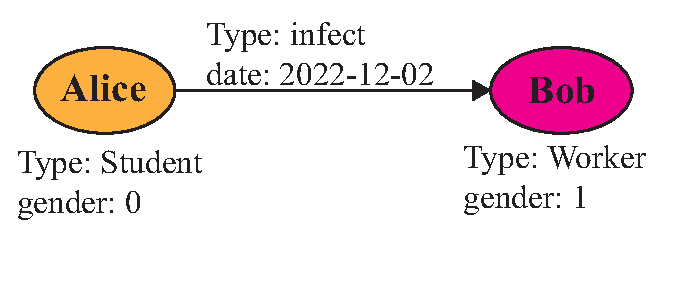
\includegraphics[width=0.45\textwidth]  {figures/propertyG.eps}} 
\bicaption{一个简单的属性图示例}{A simple property graph example}
\label{propertyG}
\end{figure}

\subsection{RDF图}
RDF(Resource Description Framework,资源描述框架)主要用于表示万维网(World Wide Web)上资源之间的关联关系,它是随着语义网的发展而被提出并逐渐流行起来的。
语义网的目标是赋予万维网上的资源以计算机可以理解的元数据,RDF的作用就是使用一种基于图的数据模型来表示万维网上不同资源之间的关系。
RDF数据集的基本组成单元是三元组;每个三元组都由主语(subject)、谓词(predicate)和宾语(object)三个部分组成,可以用 <s, p, o> 的形式来表示。
三元组中的 s 和 o 对应图中的顶点,每个三元组对应图中的一条从顶点 s 指向顶点 o 的一条类型为 p 的有向边。
此外,RDF标准还包含一些预定义的规则,例如使用谓词\texttt{rdf:type}来描述资源的类型。
图\ref{rdf}是一个简单的RDF数据集,它由7个三元组组成,其中4个三元组用于描述资源的类型,3个三元组用于描述资源间的关系。
它对应的RDF图包含四个顶点和三条边。

\begin{figure}[htb]
\centering
\begin{minipage}{.32\linewidth}
\centering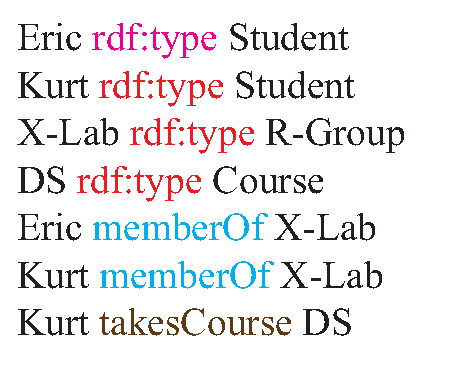
\includegraphics[scale=0.5]{figures/rdfdata.eps}
\end{minipage}
\begin{minipage}{.53\linewidth}
\centering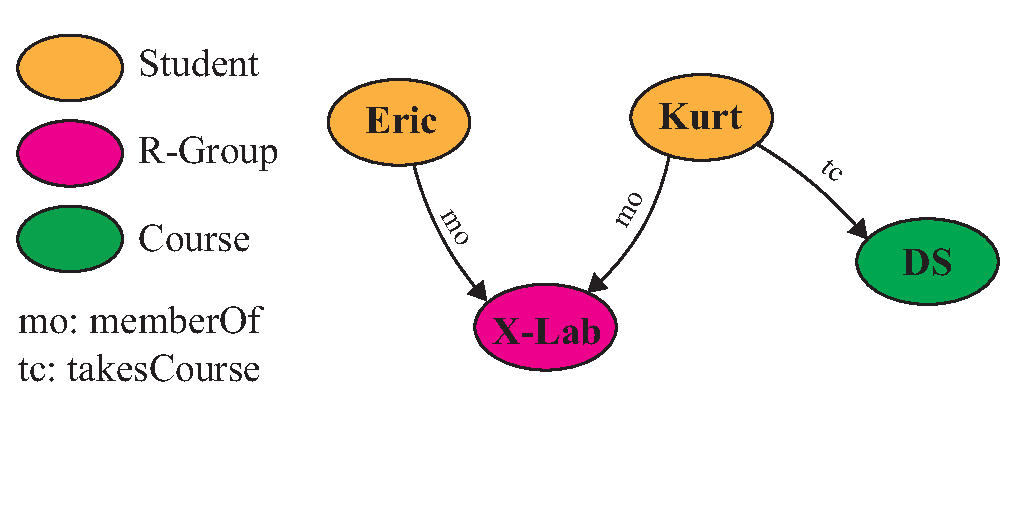
\includegraphics[scale=0.5]{figures/rdf.eps}
\end{minipage}
%\hspace*{2mm}
\begin{minipage}{1\linewidth}
\bicaption{RDF图示例}{An example of RDF graph}
\label{rdf}
\end{minipage}
\end{figure}

SPARQL\upcite{sparql}是RDF图的标准查询语言,一条 SPARQL 查询语句通过指定一个图模式来从 RDF 图中寻找与之匹配的子图。
SPARQL查询语句最常用的形式为:
\begin{eqnarray}
    \mathtt{SELECT \ RD \ WHERE \ GP}
\end{eqnarray}

其中GP是一组“主语-谓词-宾语”三元模式(TP),RD(Result Description,结果描述)是一组变量。
三元模式的每个元素都既可以是变量,也可以是常量。
除了三元模式外,GP中还可以包含过滤器,过滤器的作用是对变量的取值按照一定条件进行过滤。
RD是GP中变量的非空子集,告诉SPARQL执行引擎应该输出哪些变量的取值。
给定一个RDF图$G$和一个SPARQL查询语句$Q$,SPARQL执行引擎会在$G$上搜索与$Q$的GP匹配的子图,找到RD中所有变量的可取值。

图\ref{sparql}(a)给出了一条示例SPARQL查询语句,它想要找到满足如下条件的资源Y:Y的类型是课程且有X-Lab的成员选修该课程。
在图\ref{rdf}中寻找与图\ref{sparql}(b)所示的查询图相匹配的子图,最终可以得到如图\ref{sparql}(c)所示的查询结果。
由于RD只包含一个变量Y,所以查询结果仅有一列,变量Y仅可以取值DS,所以查询结果只有一行。

\begin{figure}[htb] 
\center{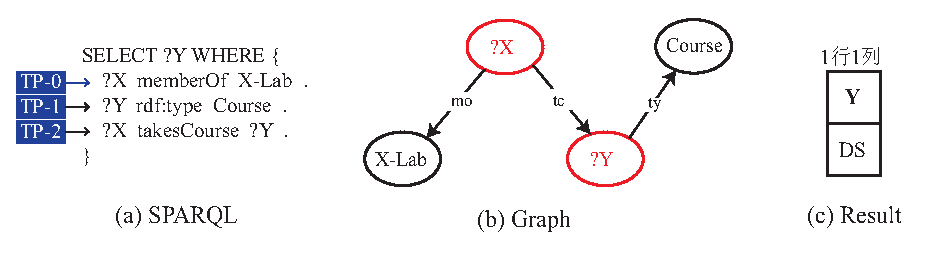
\includegraphics[width=0.9\textwidth]  {figures/sparql.eps}} 
\bicaption{示例RDF图上的一条SPARQL查询语句}{A SPARQL query statement on the RDF graph example}
\label{sparql}
\end{figure}

\subsection{超图}
超图(hypergraph)是在图的基础上泛化的一种数据结构。
普通图中的边只能与两个顶点相连接,而超图中的边能够连接任意数量的顶点。普通图只能描述二元关系,
超图能够描述多元关系。超图同样可以使用$G=(V,E)$来表示,其中$V$是超图中顶点的集合,$E$是超边的集合。
每条超边都是$V$的一个非空子集,它规定了这个集合中包含的所有顶点之间的关系。
事实上,无向图就是一种特殊的超图,这种超图的每条超边都只连接两个顶点。
类似于属性图,超图中的顶点和超边都可以拥有类型和属性。

超图非常适合用来表示可以抽象成集合的数据,例如,一个微信群聊中通常包含几个到几百个微信用户,我们可以把微信群聊抽象为超
边,把微信用户抽象为顶点,如果一个微信用户是某个群聊的成员,那么它对应的顶点就是该群聊对应超边连接的顶点之一。
图\ref{hyper}所示的超图包含 7 个顶点和 3 条超边,群聊$e_1$包含$u_1$和$u_2$两个微信用户,
群聊$e_2$包含$u_2$、$u_3$、$u_4$和$u_5$四个微信用户,$u_2$是这两个群聊的公共成员。

\begin{figure}[htb] 
\center{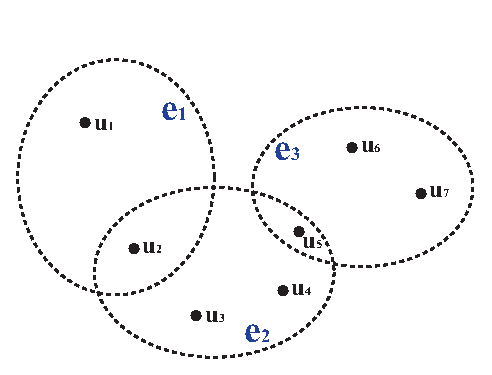
\includegraphics[width=0.4\textwidth]  {figures/hyper.eps}} 
\bicaption{用超图表示的微信群聊关系}{WeChat group relationship represented by hypergraph}
\label{hyper}
\end{figure}

\section{时序图}
属性图、RDF图和超图模型都有各自的时序版本。

在时序属性图中,顶点、边、顶点的各属性和边的各属性都可以有对应的生命周期,这样,顶点和边就可以被添加和删除,顶点和边上的属性在不同的时期也可以有不同的值。
时序属性图的正式定义为:

\begin{definition}[时序属性图]
  时序属性图可以表示为$G=(V,E)$,其中$V$是顶点$v=(vid, \tau_v)$的集合($vid$是其唯一ID,$\tau_v=[t_s, t_e)$是其生命周期时间区间),$E$是边$e=(eid, uid, vid, \tau_e)$的集合($eid$是其唯一ID,$uid, vid\in V$分别是其起点和终点,$\tau_e=[t_s', t_e')$是其生命周期时间区间)。
\end{definition}

时序属性图需要满足一个完整性约束:边的生命周期不能超出它所连接的两个顶点的生命周期。
图\ref{interval}给出了一个满足完整性约束的时序属性图示例,它包含五个顶点和六条边。顶点的生命周期都是$[0,10)$,不同边的生命周期不尽相同,例如顶点$A$和顶点$B$之间有两条边,生命周期为$[0,1)$的边的属性值为$3$,生命周期为$[1,4)$的边的属性值为$7$。

\begin{figure}[htb] 
\center{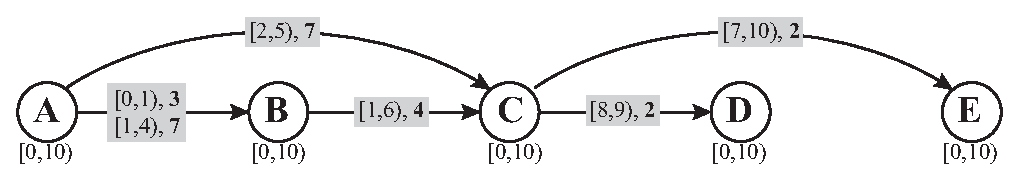
\includegraphics[width=0.9\textwidth]  {figures/interval.eps}} 
\bicaption{时序属性图示例}{An example of temporal property graph}
\label{interval}
\end{figure}

时序RDF图并没有统一的标准定义,结合之前工作对时序RDF图的定义,本文把时序RDF图定义为:

\begin{definition}[时序RDF图]
  时序三元组是带有整数有效时间标签的三元组,可以表示为$(s,p,o):[t]$。时序RDF图就是时序三元组的集合。
  我们使用$(s,p,o):[t_1,t_2)$来简记$\{(s,p,o):[t]|t_1\leq t<t_2,t\in Z\}$,它表示三元组$(s,p,o)$在$[t_1,t_2)$这个时间区间上是有效的。
\end{definition}

图\ref{trdf}是一个时序RDF数据集示例,它是图\ref{rdf}中的RDF图的时序版本,由7个时序三元组组成。
它构成的时序RDF图包含三条边,这三条边都有各自的有效时间区间,例如Eric和X-Lab之间的边的有效时间区间是$[1,2)$。

\begin{figure}[htb]
\centering
\begin{minipage}{.35\linewidth}
\centering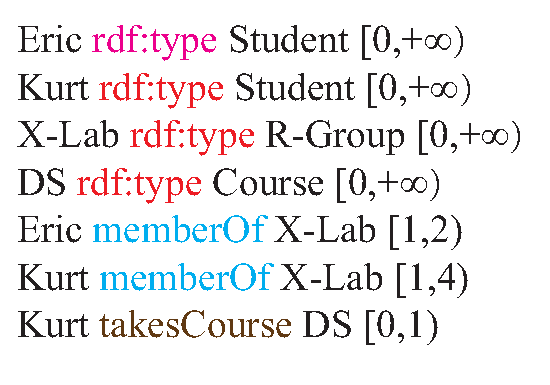
\includegraphics[scale=0.5]{figures/trdfdata.eps}
\end{minipage}
\begin{minipage}{.55\linewidth}
\centering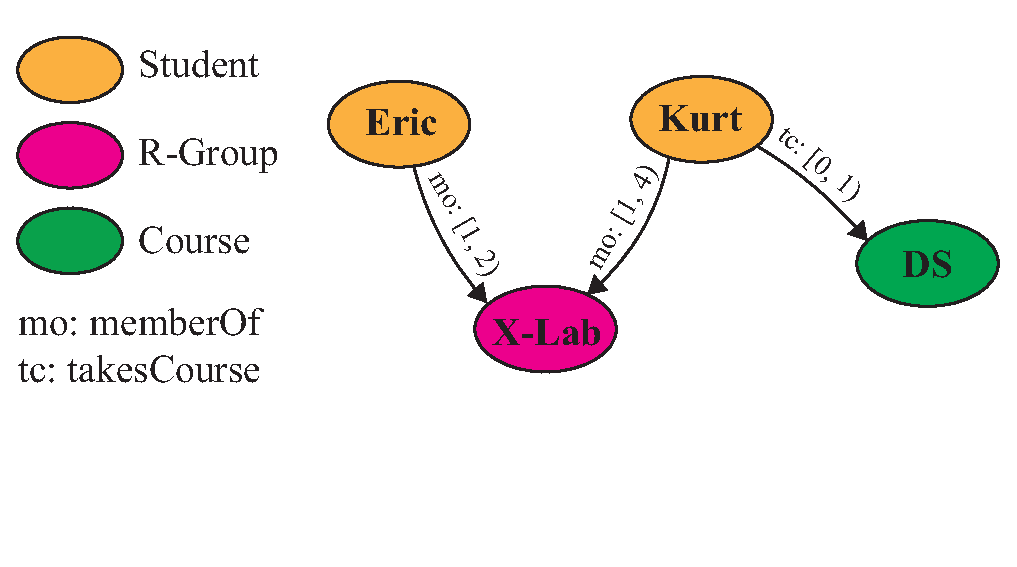
\includegraphics[scale=0.5]{figures/trdf.eps}
\end{minipage}
%\hspace*{2mm}
\begin{minipage}{1\linewidth}
\bicaption{时序RDF图示例}{An example of temporal RDF graph}
\label{trdf}
\end{minipage}
\end{figure}

时序超图同样没有标准的定义,本文把时序超图定义为:

\begin{definition}[时序超图]
  顶点集合$V=\{v_1,...,v_{|V|}\}$上的时序超图$G=(V,E)$是一个时序超边的集合$E=\{e_1,...,e_{|E|}\}$,
  每条时序超边$e=\widetilde{e}:[t]\in E $都是一个带有整数有效时间标签$t$的顶点集合$V$的非空子集。
  我们使用$\widetilde{e}:[t_1,t_2)$来简记$\{\widetilde{e}:[t]|t_1\leq t<t_2,t\in Z\}$,
  它表示时序超边$\widetilde{e}$在$[t_1,t_2)$这个时间区间上是有效的。
\end{definition}

在时序超图中,时序超边和顶点都是可以有类型的。图\ref{thyper}是一个时序超图示例,它是图\ref{hyper}中超图的时序版本,它包含三条时序超边,都有各自的有效时间区间,例如$e_1$表示的微信群聊状态只在时间区间$[1,3)$内是成立的。

\begin{figure}[htb] 
\center{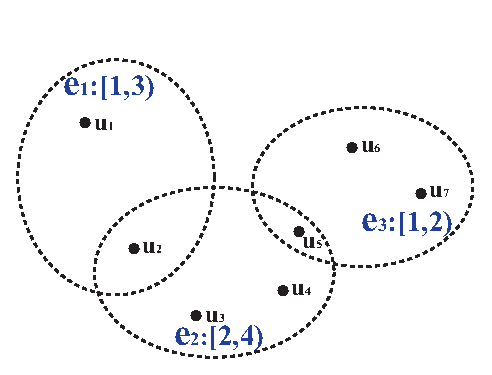
\includegraphics[width=0.4\textwidth]  {figures/thyper.eps}} 
\bicaption{用时序超图表示的微信群聊关系}{WeChat group relationship represented by temporal hypergraph}
\label{thyper}
\end{figure}

\section{Wukong介绍}
\sys 的时序图查询模块是在Wukong的基础上实现的。
Wukong是一个先进的分布式RDF图查询系统,它基于RDMA这一新型硬件特性,通过一系列存储结构和查询引擎上的优化技术,实现了SPARQL查询的低时延、高并发执行。

RDMA(Remote Direct Memory Access,远端内存直接访问)是一种高性能的跨机器内存访问技术,能够以很低的延迟直接访问远端机器的内存。
RDMA操作主要分为两类:单边(one-sided)操作和双边(two-sided)操作。
单边操作可以不经过远端机器的CPU直接读、写其内存,也不需要操作系统内核的参与。
双边操作类似于传统消息传递模式,即分别使用SEND和RECV两个接口进行消息的发送和接收。
虽然双边操作需要服务端CPU的参与,但由于双边操作中的网络协议栈完全由支持RDMA的网卡硬件实现,因此相较于传统基于TCP/IP协议的消息传递,RDMA双边操作仍然能有超过一个数量级的性能提升。

接下来,本文将从存储结构和查询引擎两个方面对Wukong作简要介绍。

\begin{figure}[htb]
\center{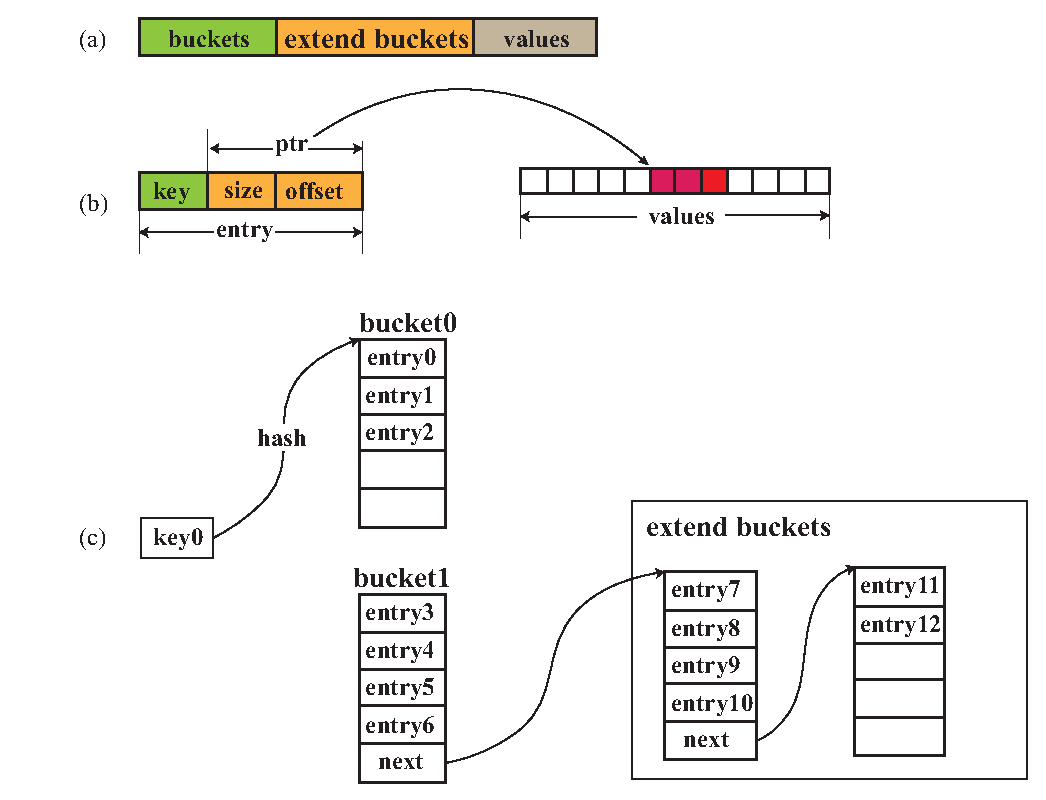
\includegraphics[width=0.8\textwidth]  {figures/kvstore.eps}} 
\bicaption{Wukong的分布式键值存储结构}{Wukong's distributed key-value store structure}
\label{kvstore}
\end{figure}

\subsection{存储结构}
\label{chap:kvstore}
为了充分发挥RDMA在远端内存访问上的性能优势,Wukong使用多机内存实现RDF图数据集的可扩展存储,使用单边RDMA操作访问远端机器的内存。Wukong的基本存储结构是一个如图\ref{kvstore}的分布式键值存储结构。
每台机器上的键值存储由图\ref{kvstore}(a)所示的三块连续的内存区域组成,其中buckets和extend buckets是键和它对应值的位置信息的存储区域,values是值的存储区域。
一个键和它对应值的位置信息组成一个图\ref{kvstore}(b)中的entry,其中key是键本身,size和offset分别是该键对应值的长度(值是一个列表)和位置(相对于values区域起始位置的偏移量)。
如图\ref{kvstore}(c)所示,buckets和extend buckets区域由一系列桶(bucket)组成,每个桶都有$N$个槽(slot),最多可以容纳$N-1$个entry。
给定一个key,系统会使用一个哈希函数计算它对应的entry应该被放在buckets区域中的哪个桶里,当桶满(同一哈希值的key的数量超过$N-1$)时,系统会从extend buckets里分配新桶来继续存放剩下的条目,满桶的最后一个槽会被用来存放指向新桶的指针,形成一个类似于链表的结构。

\begin{algorithm}[htb]
\caption{根据给定键读取对应值}
\label{algo:readkv}
\SetKwInOut{Input}{输入}
\SetKwInOut{Output}{输出}
\SetKw{KwTo}{in}
\SetKwFunction{Range}{range}
\SetKwFor{For}{for}{\string:}{}
\SetKwIF{If}{ElseIf}{Else}{if}{:}{elif}{else:}{}
\SetKwFor{While}{while}{:}{}
\newcommand{\forcond}{$i$ \KwTo\Range{$N$}}
\Input{key}
\Output{值数组}
server\_id $\leftarrow$ hash\_server(key)\;
bucket\_id $\leftarrow$ hash\_bucket(key)\;
slot $\leftarrow$ NULL\;
\While{true}{
    rdma\_offset $\leftarrow$ bucket\_id $\times N \times$ sizeof(slot)\;
    rdma\_size $\leftarrow$ $N \times$ sizeof(slot)\;
    slots $\leftarrow$ RdmaRead(server\_id, rdma\_offset, rdma\_size)\;
    \For{\forcond}{
        \If{$i<N$}{
            \If{slots[$i$].key = key}{
                slot $\leftarrow$ slots[$i$]\;
                goto $read$\;
            }
        }
        \Else{
            \If{IsEmpty(slots[$i$])}{
                goto $read$\;
            }
            bucket\_id $\leftarrow$ slots[$i$].bid\;
        }
    }
}
$read:$
\BlankLine
    \If{slot = NULL}{
        \Return $[]$\;
    }
    \Else{
        \Return RdmaRead(server\_id, values\_base + slot.offset $\times$ sizeof(value), slot.size $\times$ sizeof(value))\;
    }
\end{algorithm}

算法\ref{algo:readkv}给出了根据给定key读取对应值的伪代码。系统首先会通过两个哈希函数计算该key会被存储在哪台机器的哪个桶里(1-2行),然后通过RDMA的单边读操作从相应机器把整个桶都读取过来(5-7行),遍历桶的前$N-1$个槽,对比每个entry的key是否和给定key匹配,如果找不到一致的entry,则通过第N个槽提供的指针继续查找extend buckets区域里的槽(16行),直到寻找到匹配的entry或扫完最后一个桶。
如果搜索到匹配的entry,直接通过RDMA的单边读操作从相应机器的values区域的正确位置读取值即可(21行)。

\subsection{查询引擎}
\label{chap:engine}
Wukong的查询执行引擎使用图探索和全历史剪枝算法执行SPARQL语句。
以图\ref{sparql}中的查询语句为例,图\ref{engine}展示了该语句的执行过程。
查询引擎依次处理语句中的三元模式(\ding{182}),对于每个三元模式,查询引擎会通过构造合适的key从系统的分布式键值存储中查找与该三元模式匹配的子图,这一过程称为图探索。
每个子图都对应着查询语句中变量的一组取值,执行完每个三元模式后探索到的所有子图对应的变量的取值构成中间结果表。
所有三元模式都执行完毕后,中间结果表中RD对应的列就作为最终的查询结果返回给用户。
例如,变量$?X$和$?Y$的所有可取值在TP-1执行完毕后已经被找到,三元模式TP-2的目的是从中筛选出存在takesCourse关系的变量$?X$和$?Y$的取值。
在执行三元模式TP-2时,查询引擎会将中间结果表第一列中的每个值(变量$?X$的取值,\ding{183})分别与三元模式中的谓词常量takesCourse构成key(\ding{184}),从分布式键值存储中读取对应的值(\ding{185}),当且仅当第二列中的值出现在\ding{185}中,该行才会被保留在中间结果表中。
这种通过之前步骤的历史信息精确地修剪掉无用中间结果的的方法就是全历史剪枝。

\begin{figure}[htb]
\center{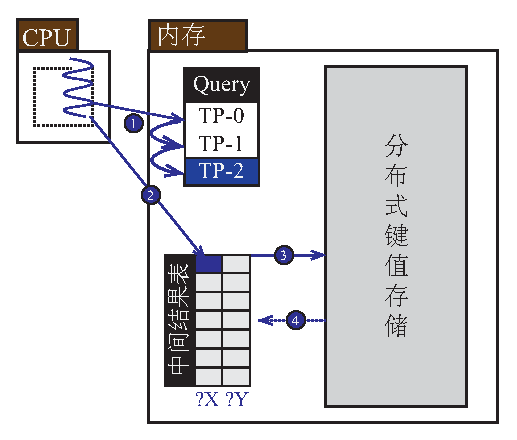
\includegraphics[width=0.5\textwidth]  {figures/engine.eps}} 
\bicaption{SPARQL查询执行过程}{SPARQL query execution process}
\label{engine}
\end{figure}

\section{图分析系统的图存储结构}
CSR (Compressed Sparse Row)是静态图分析系统广泛使用的图存储结构,它是稀疏矩阵的紧凑化表示,图\ref{csr}(a)是一个简单的图拓扑,图\ref{csr}(b)是它的CSR表示,CSR由一个顶点数组和一个边数组组成,其中边数组按照边的起点ID的顺序来存储每条边的终点ID,顶点数组通过顶点的ID来索引,它存储各个顶点的出边在边数组中起始位置的偏移量。在在线图分析场景中,图拓扑会不断更新,而CSR是一种紧凑的结构,在CSR上做图拓扑更新的效率很低,例如,如果在\ref{csr}(a)的图结构中添加一条从顶点0指向顶点3的边,它的CSR表示就需要对顶点数组和边数组做大量更新(如图\ref{csr}(c))

\begin{figure}[!htb]
\center{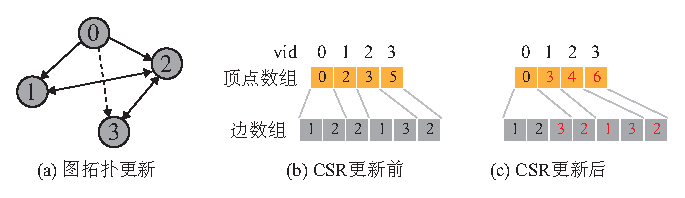
\includegraphics[width=0.8\textwidth]  {figures/csr-update.eps}} 
\bicaption{图拓扑的CSR表示}{CSR representation of graph topology}
\label{csr}
\end{figure}

在线图分析系统(例如RisGraph\cite{risgraph}、GraphOne\cite{graphone}和LiveGraph)和动态图存储(例如CSR++\cite{csrpp}和Sortledton\cite{sortledton})通常使用邻接列表作为图拓扑存储的基本数据结构。
如图\ref{adja}(a),使用邻接列表表示图拓扑时,每个顶点的所有出边的终点ID都会被存放在一个单独的邻接列表中,邻接列表指针数组存放指向每个邻接列表的指针。如图\ref{adja}(b),在添加一条从顶点0指向顶点3的边时,只需要往顶点0的邻接列表中添加一个元素3即可。逐顶点的邻边扫描(以下简称扫边)是图分析中最常用的操作。图拓扑的邻接列表表示虽然具有更高的图更新效率,但它的结构较为松散,在扫边过程中的数据局部性较差,扫边性能远不及图拓扑的CSR表示。
\begin{figure}[!htb]
\center{
\includegraphics[width=0.6\textwidth]  {figures/adja.eps}} 
\bicaption{图拓扑的邻接列表表示}{Adjacency list representation of graph topology}
\label{adja}
\end{figure}

\section{本章小结}
本章介绍了与本工作相关的背景知识。
属性图、RDF 图和超图是定义图结构的三大范式。
属性图是最为常用的建模图状结构数据的模型;
RDF的作用是使用一种基于图的数据模型来表示万维网上不同资源之间的关系,SPARQL是RDF图的标准查询语言;超图是在图的基础上泛化的一种数据结构,超图中的边能够连接任意数量的顶点。随着时间而变化的图叫做时序图,属性图、RDF图和超图都有各自的时序版本。
本文给出了时序属性图的正式定义,然后结合之前工作给出了时序RDF图和时序超图的定义。
\sys 的时序图查询模块是在Wukong的基础上实现的,本章从存储结构和查询引擎两个方面对Wukong进行了简要介绍。
CSR和邻接列表是图分析系统常用的两种图存储结构,它们分别适用于离线和在线图分析系统。